\chapter{Training details}

All experiments were carried out on the RCI (Research Center for Informatics) Cluster at the Czech Technical University in Prague.

Following Košťál et al.~\cite{Kostal2025}, we used the Adam optimizer with a learning rate $10^{-4}$ and a weight decay penalty of $10^{-5}$.
The only alternative learning rate employed was $2\cdot 10^{-4}$, used for the hard-constrained models in the resampling experiments (Section~\ref{s:resampling_method_exp}). 
This choice was made because the hard-constrained models exhibit a very smooth learning curve, whereas the other models are far less stable, making the higher learning rate unsuitable for them (see Figure\ref{fig:validation_rmse}).
Furthermore, an early stopping strategy with a patience of 15 was applied based on the validation pixel-wise RMSE, except in the experiment on model sizes (Section~\ref{s:models_size_exp}), where the patience was reduced to 10, due to the larger number of runs.

\begin{figure}[h]
    \centering
    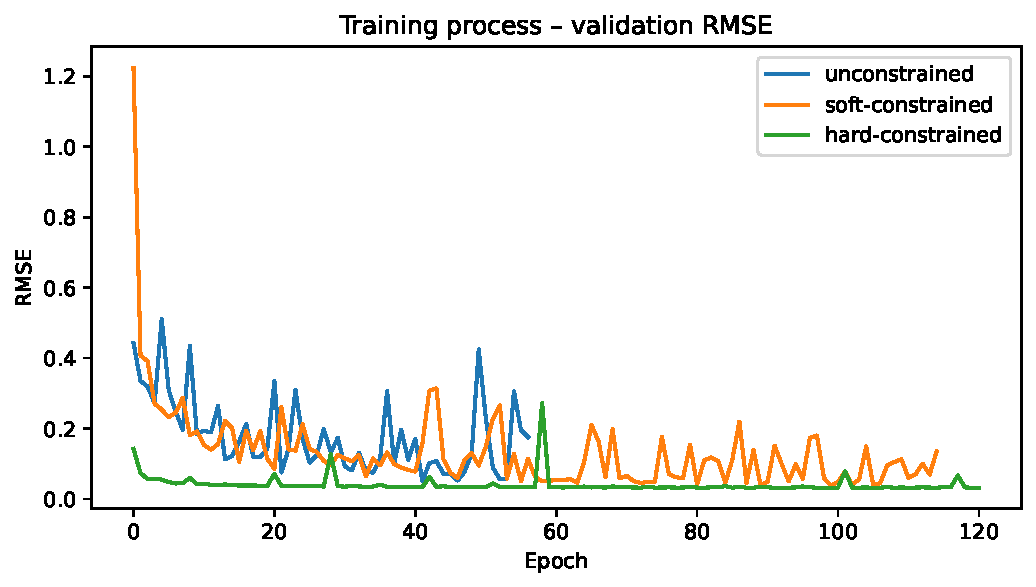
\includegraphics[width=0.7\linewidth]{images/validation_rmse.pdf}
    \caption[Training process]{Training process. 
    An unconstrained a conservation soft-constrained and a conservation hard-constrained models validation pixel-wise RMSEs are shown through the learning process. 
    All the models are EDSR with 128 features and 64 residual blocks. 
    The unconstrained and the soft-constrained model have Adam optimizer with the learning rate of $10^{-4}$, whereas the hard-constrained model has $2\cdot 10^{-4}$, yet it appears to be more stable through the learning.}
    \label{fig:validation_rmse}
\end{figure}

\chapter{Image comparisons}

In Chapter~\ref{ch:experiments} various experiments have been concluded on ReKIS data.
However, only a numerical evaluation of the employed models took place via MAE or RMSE metrics.
Now we present the visual distinctions between the selected models.
In every visualization, the LR model input and the corresponding HR target are displayed.
First, the entire area is shown, followed by a blue square highlighting a zone where elevation, and thus the temperature, are steadier.
Lastly, the red square marks an area characterized by strong temperature variations.

\begin{landscape}
    \begin{figure}
    \centering
    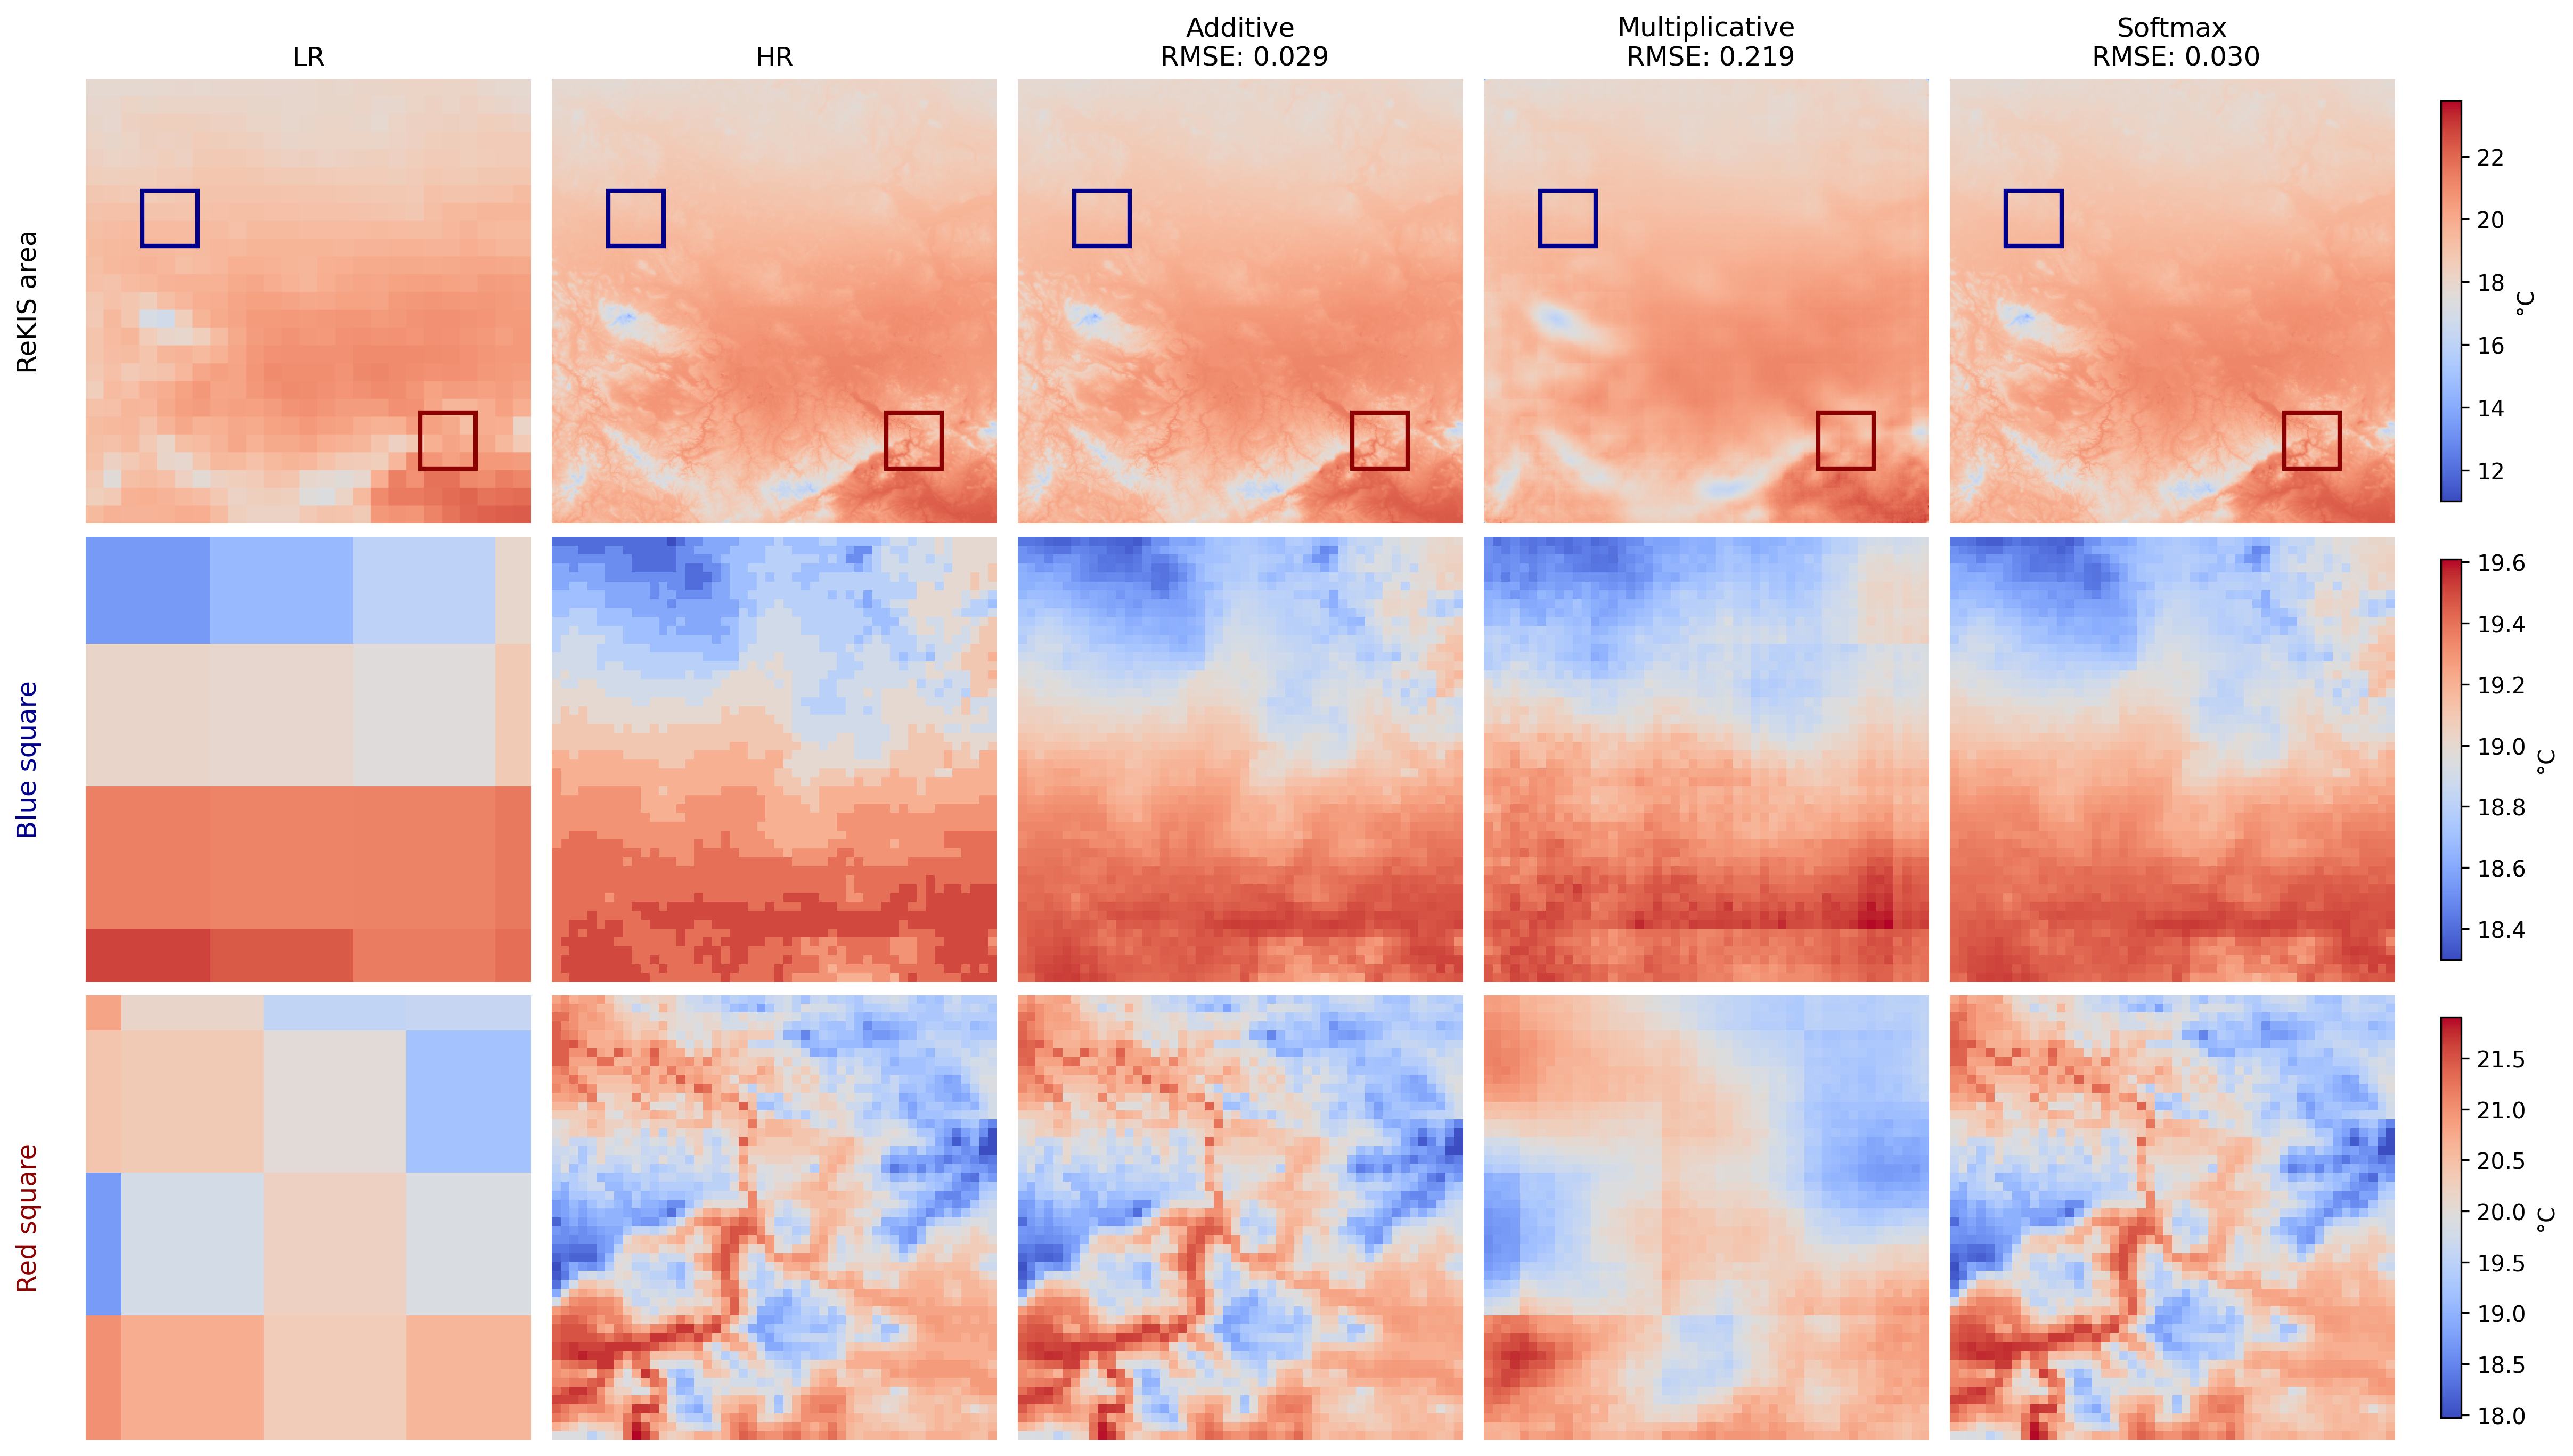
\includegraphics[width=0.88\linewidth]{images/hard_types_comp.png}
    \caption[Hard-constrained model types -- output visual comparison]{
    Hard-constrained model types -- output visual comparison. 
    The models are from Section~\ref{s:hard_constraint_exp}. 
    The multiplicative hard-constraint layer is significantly different than the other implementations -- the larger LR pixels are visible in the blurred output. 
    The HR image in the blue square displays artifacts that look as if it has been rounded or truncated to a fixed number of decimal places. 
    The additive and the softmax approaches are almost identical.
    Images correspond to the date 2005-08-18.}
    \label{fig:hard_types_comp}
\end{figure}
\end{landscape}

\begin{landscape}
    \begin{figure}
        \centering
        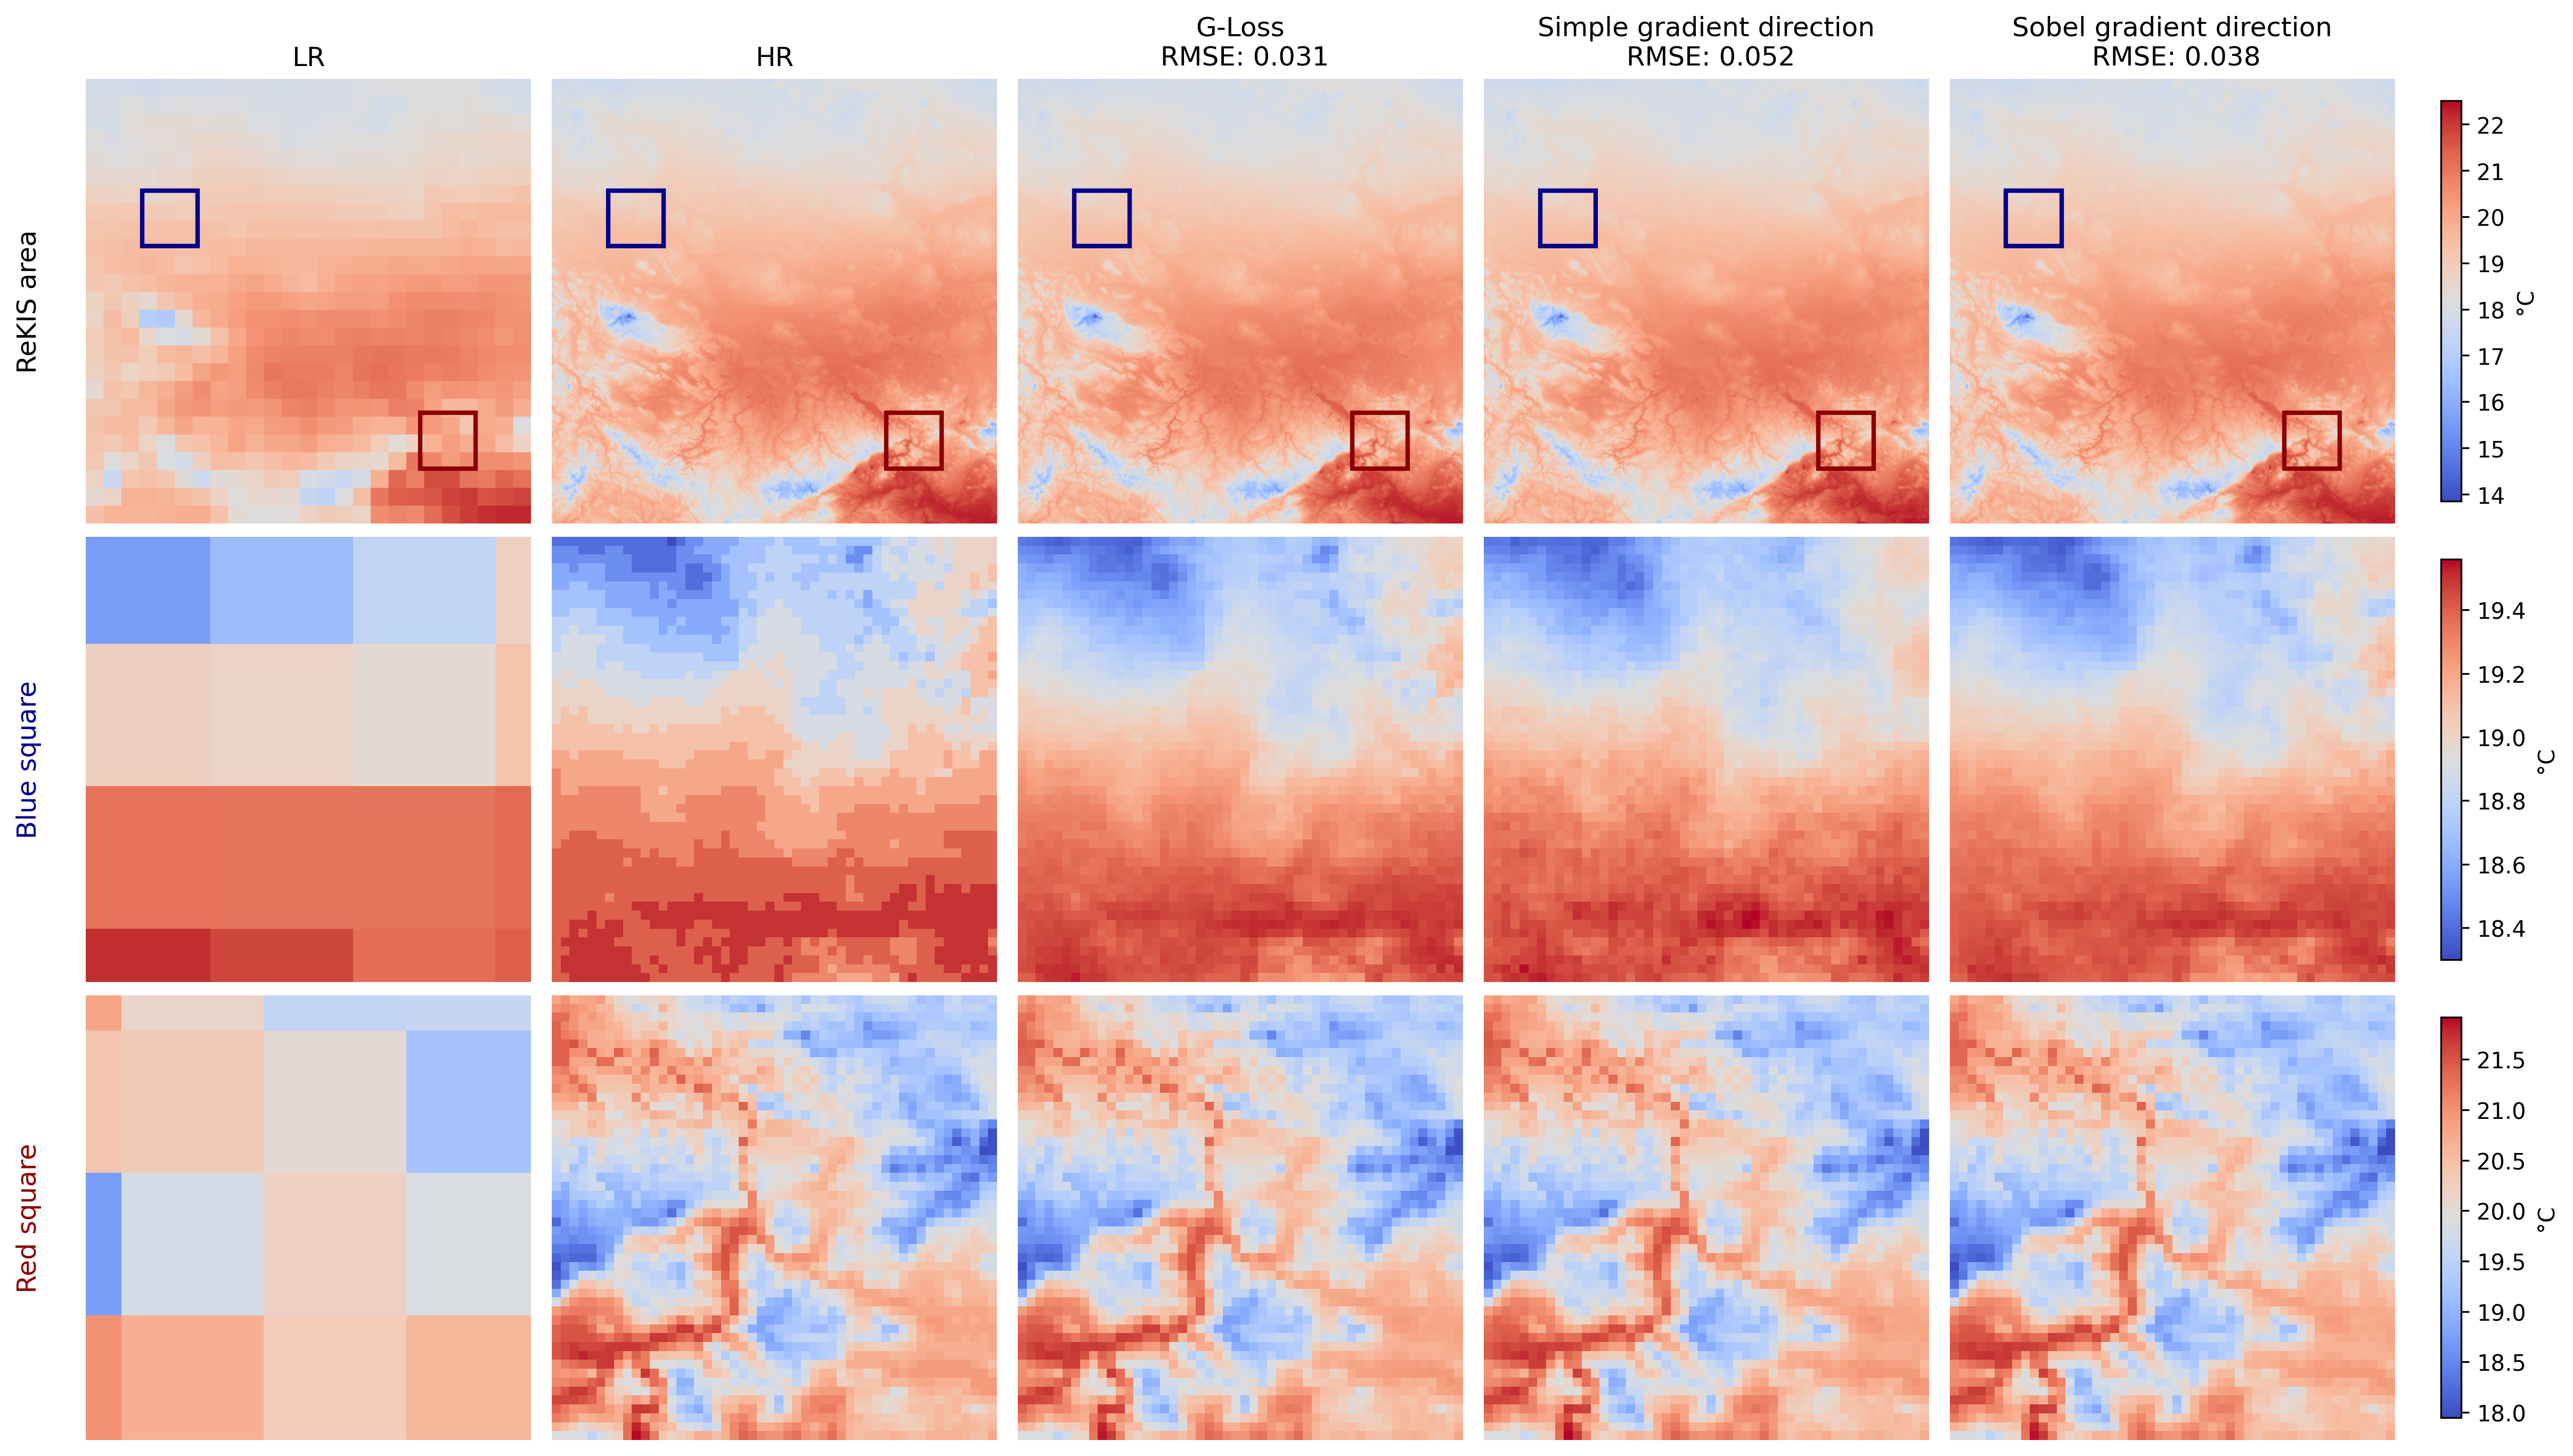
\includegraphics[width=0.88\linewidth]{images/soft_types_comp.png}
        \caption[Soft-constrained model types -- output visual comparison]{
        Soft-constrained model types -- output visual comparison. 
        The models are from Section~\ref{s:constraints_exp}. 
        The soft constraint on the gradient direction when using simple kernels results in a noisy output, as seen in the blue square. 
        In contrast, the Sobel variant generates a more compact result. This can be caused by the derivative kernels: Sobel kernels capture information over a larger neighborhood, making them more robust to noise. 
        G-Loss and Sobel gradient direction constraints are almost identical, however the G-Loss produces slightly more intense outputs in the top right corner of the blue square.
        Images correspond to the date 2005-08-18.}
        \label{fig:soft_types_comp}
    \end{figure}
\end{landscape}


\begin{landscape}
    \begin{figure}
    \centering
    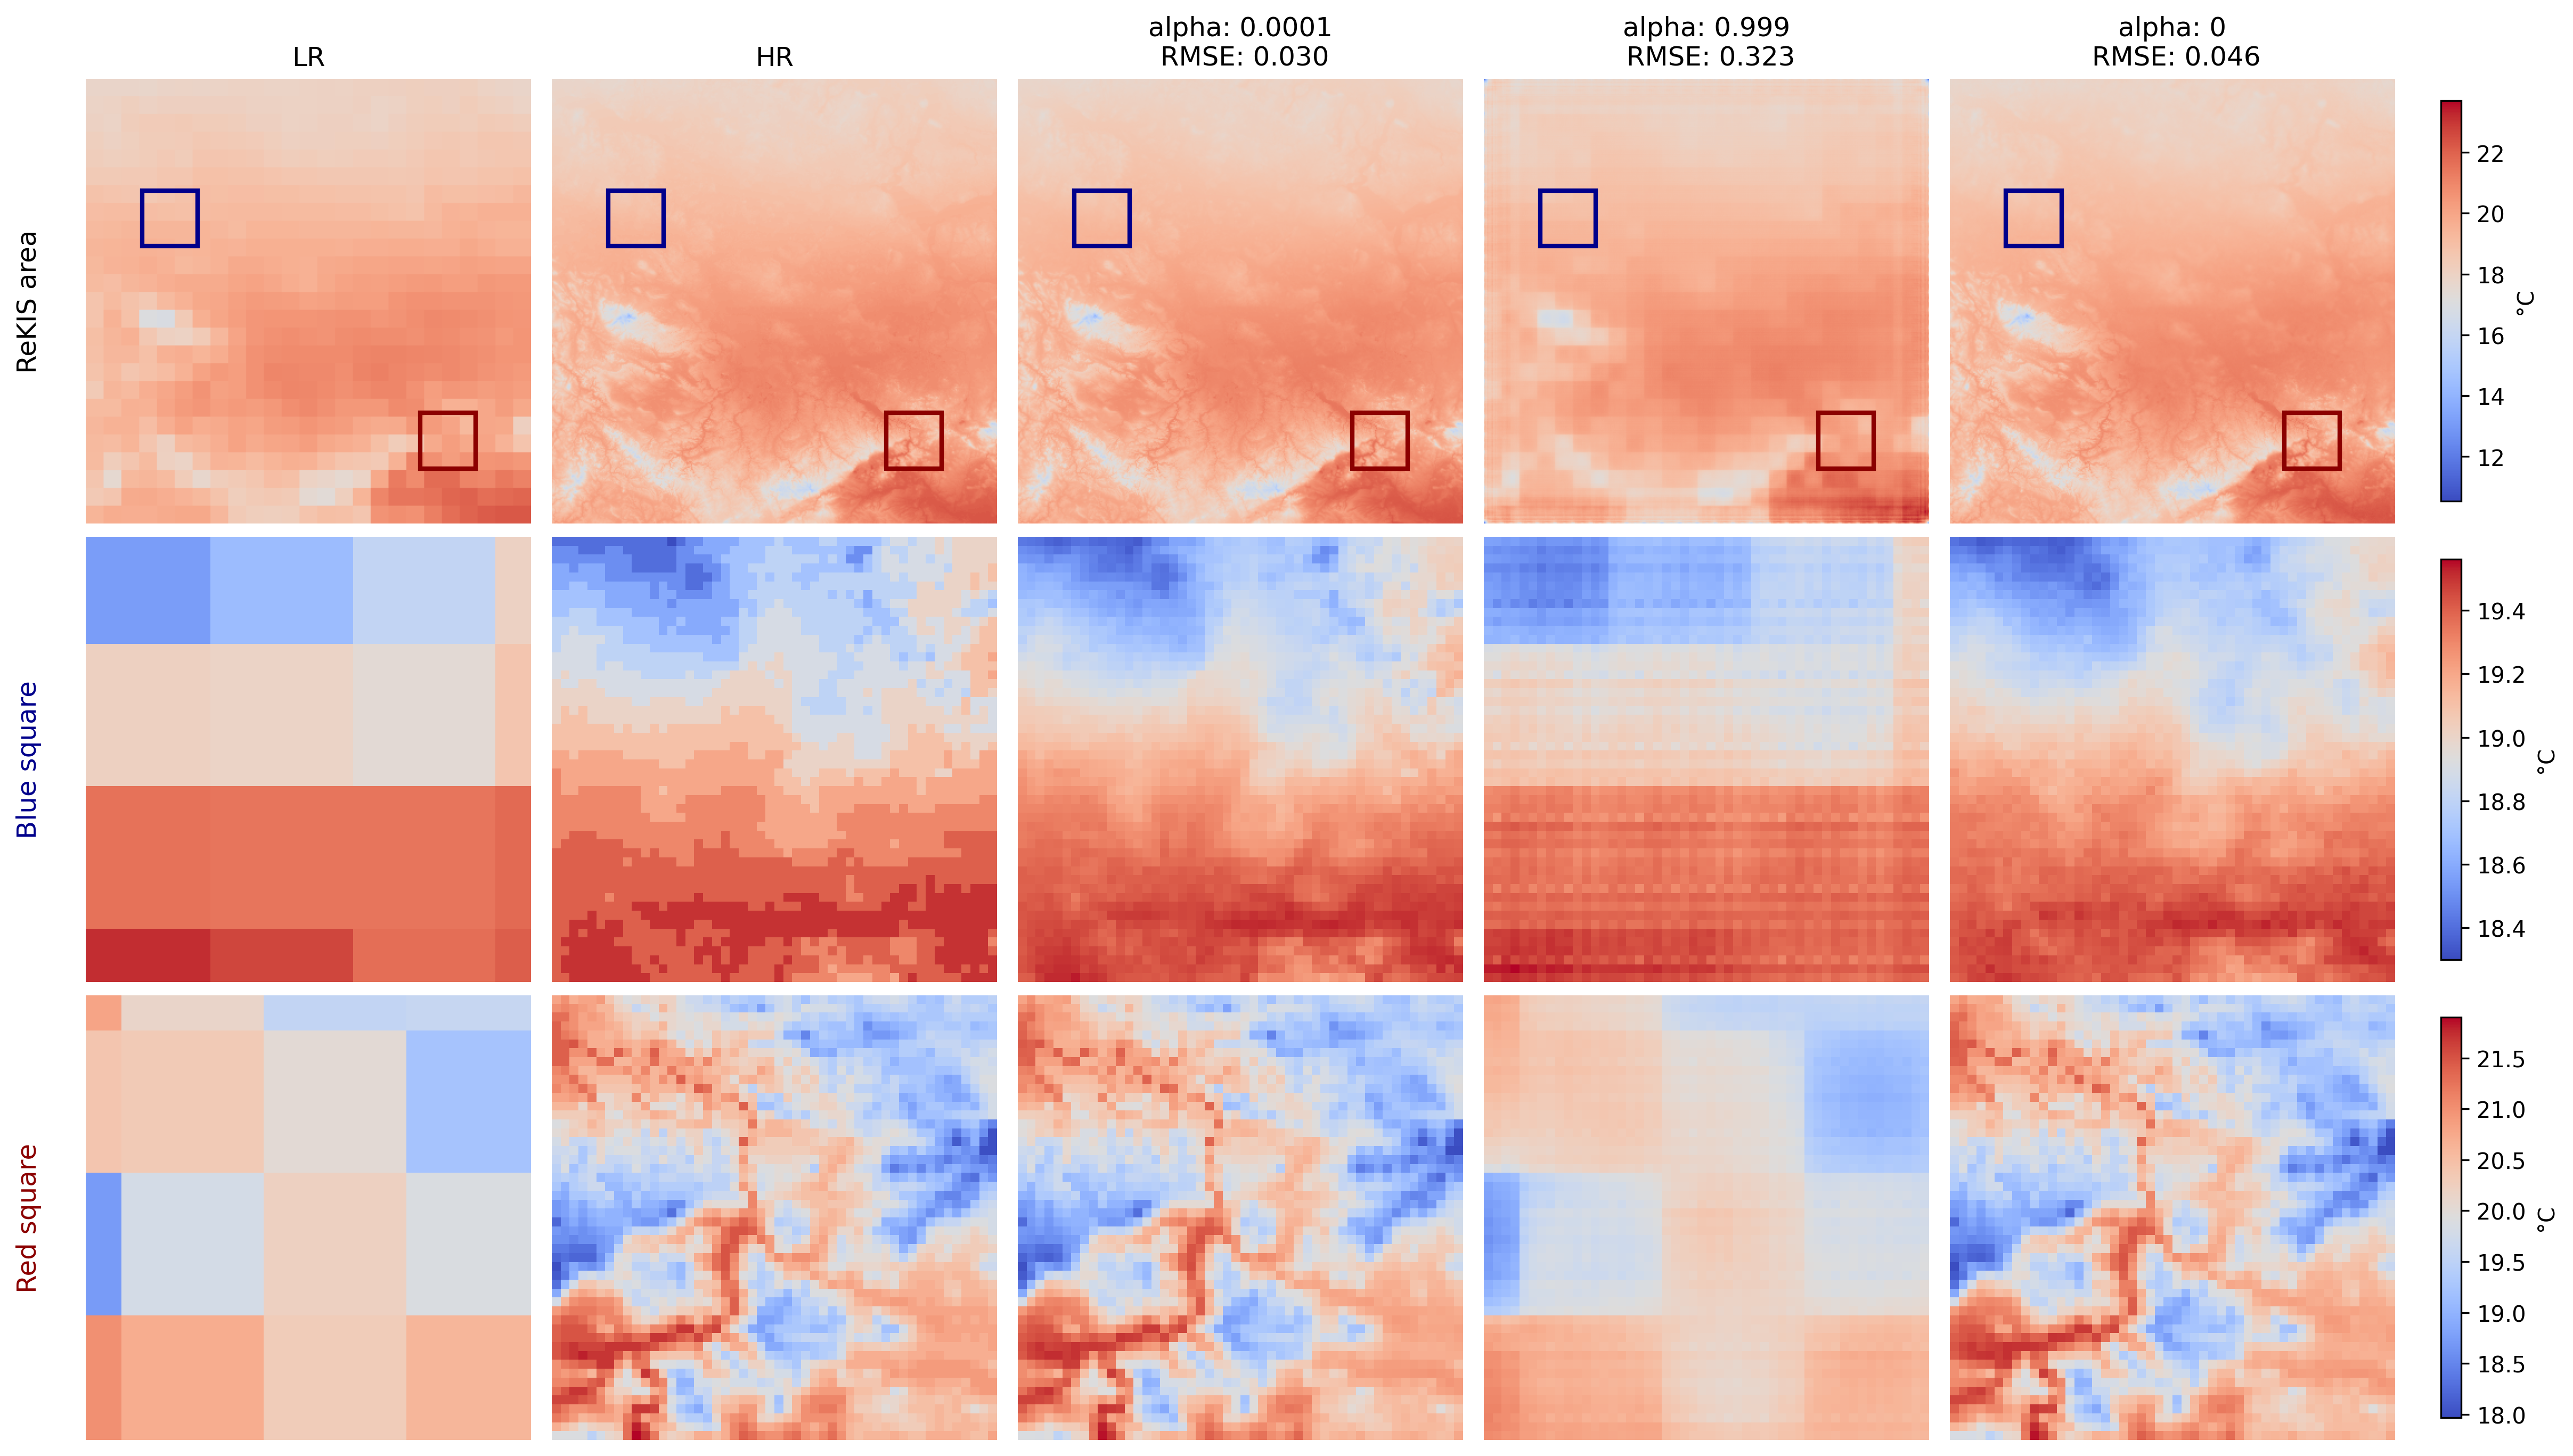
\includegraphics[width=0.88\linewidth]{images/alphas_comp.png}
    \caption[Alpha values experiment -- output visual comparison]{
    Alpha values experiment -- output visual comparison. The models are from Section~\ref{s:soft_constraints_alpha_exp}. 
    The model with alpha equal to 0.999 is producing noisier LR-like output. 
    A too large alpha value forces the model to strictly preserve the average between pixels, which results in merely reproducing the input, since the pixel-wise error contributes only weakly to the loss function. 
    The blue area of the model with alpha set to 0.0001 appears slightly more intense, than in the unconstrained model, particularly in the upper-right corner where three blue dots are located.
    Images correspond to the date 2005-08-18.}
    \label{fig:alphas_comp}
\end{figure}
\end{landscape}

\begin{landscape}
    \begin{figure}
    \centering
    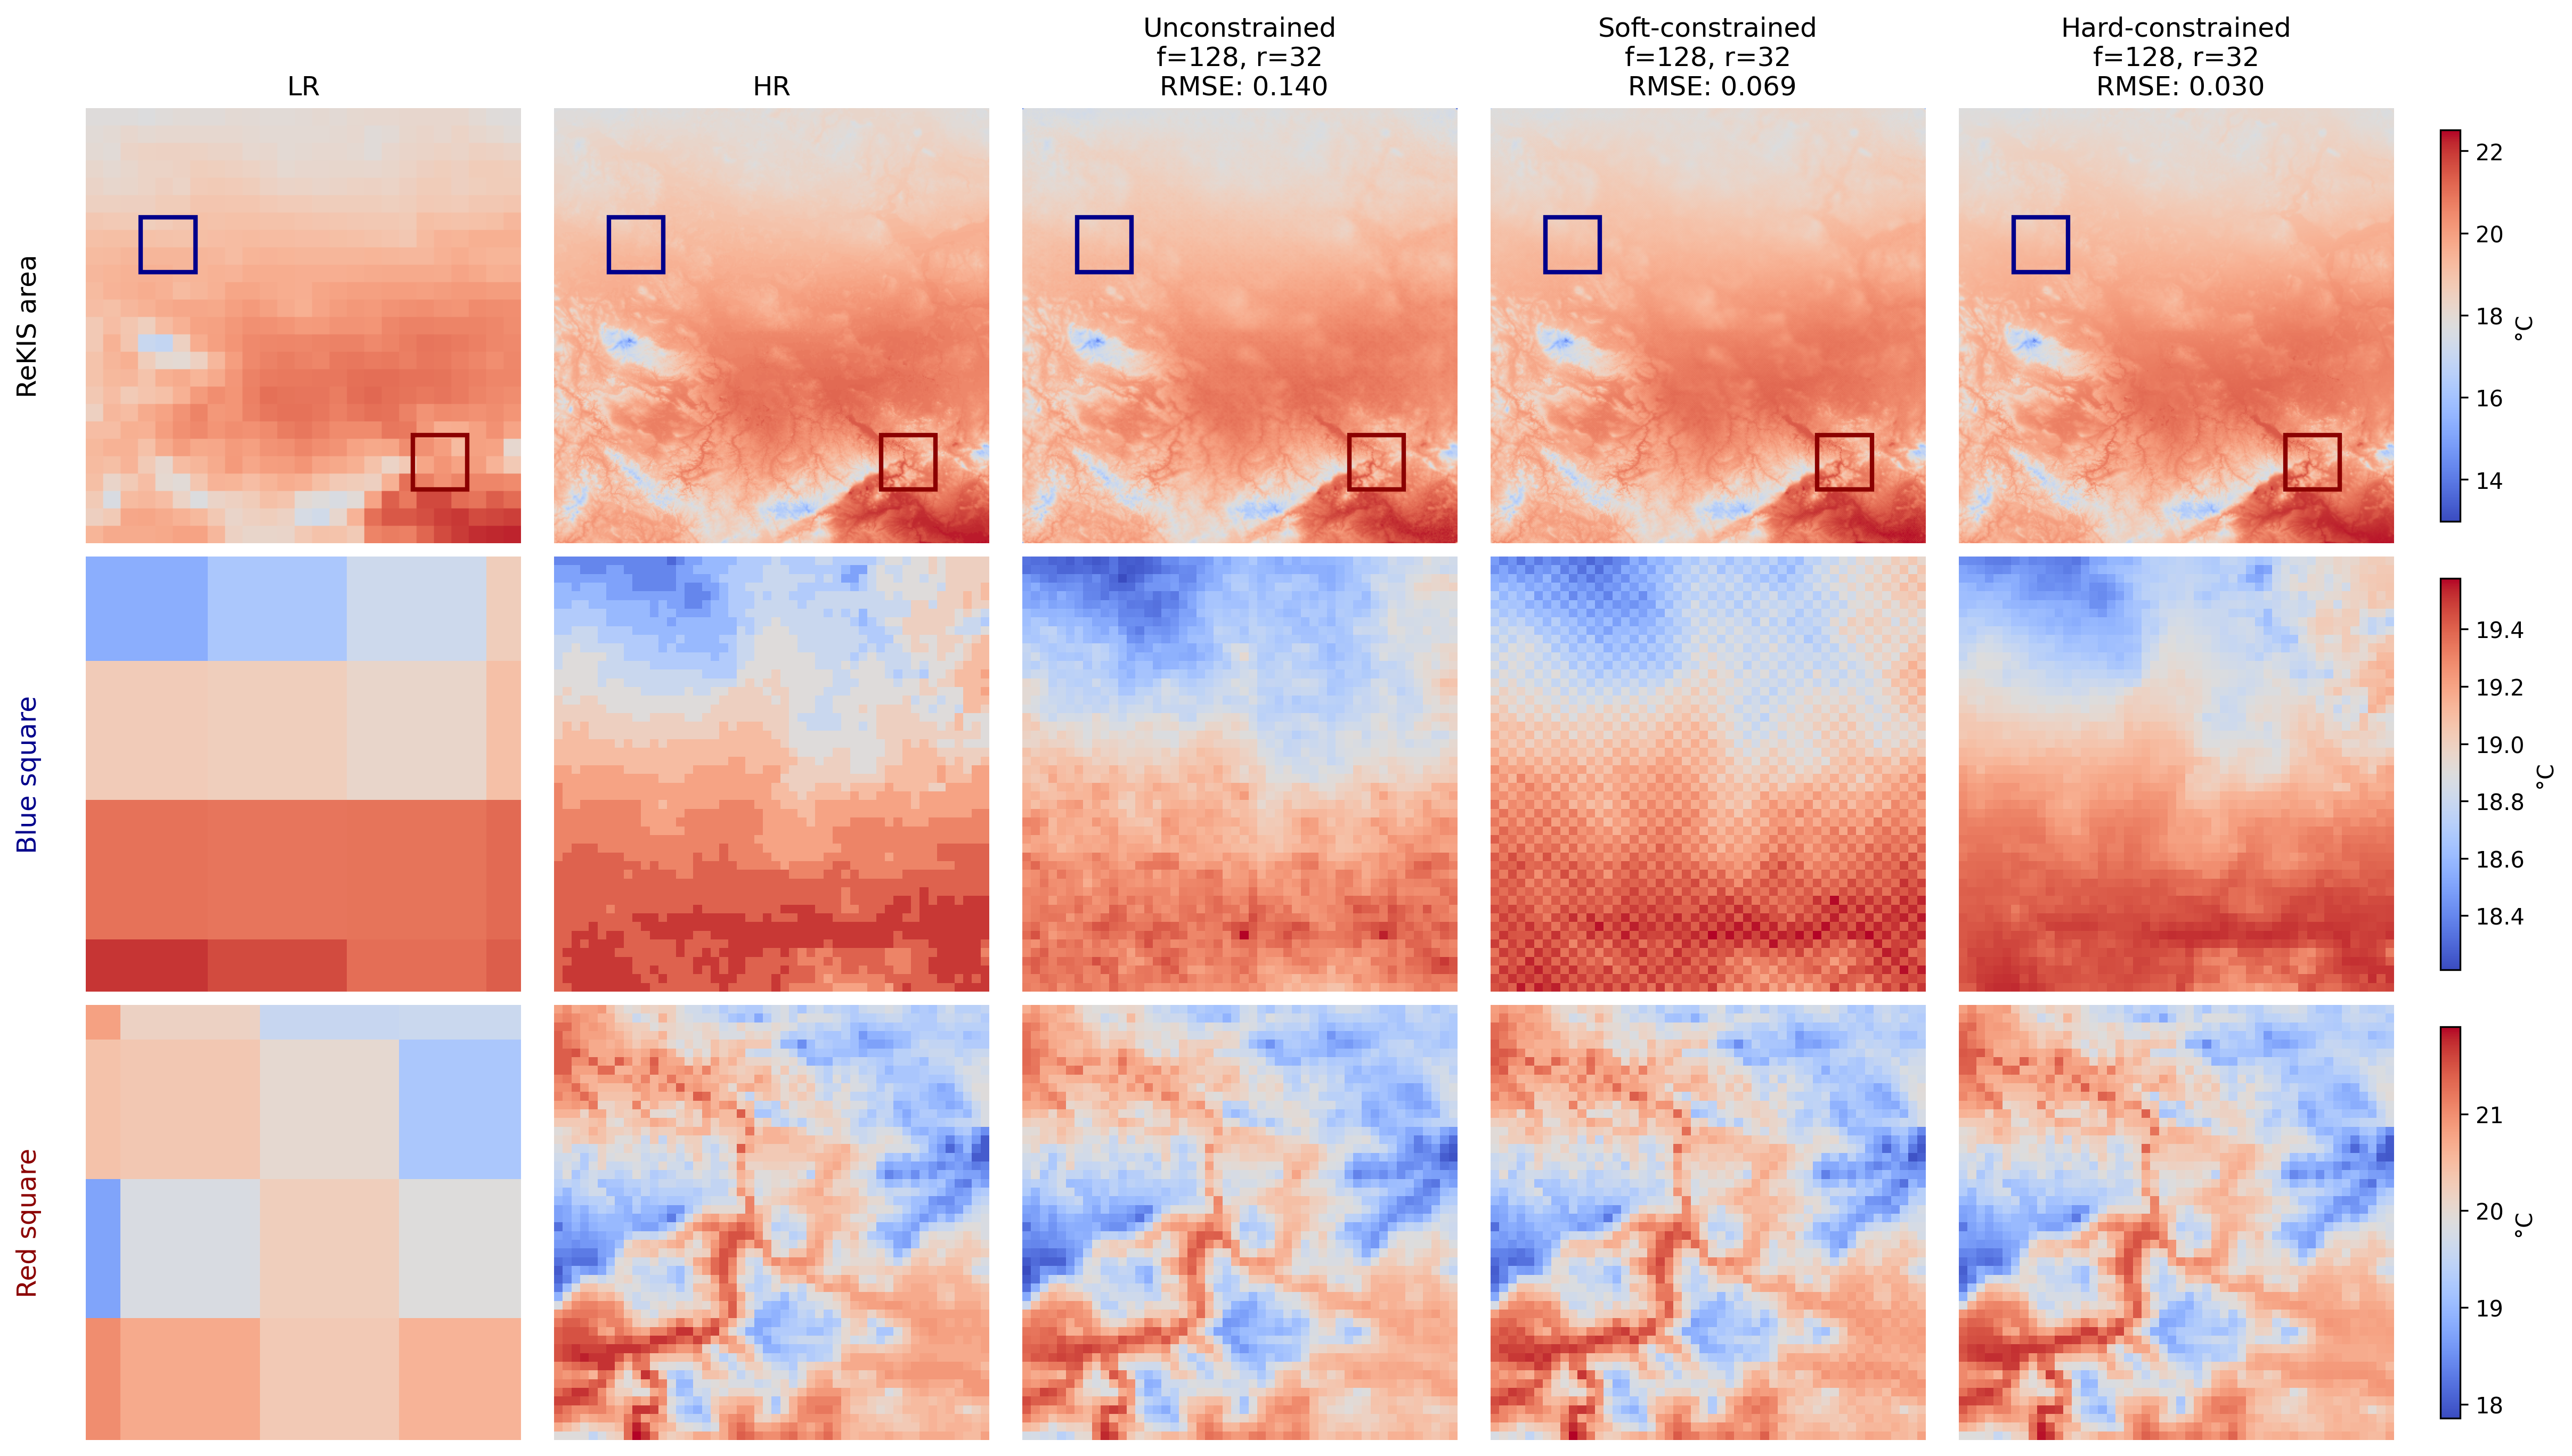
\includegraphics[width=0.88\linewidth]{images/constraint_type_comp.png}
    \caption[Constraint types -- output visual comparison]{
    Constraint types -- output visual comparison. The models are from Section~\ref{s:models_size_exp}. 
    Graining can be observed in the outputs of both the unconstrained and soft-constrained models. 
    In the unconstrained setting, the this looks like random noise, whereas under the soft-constraint it becomes more structured, almost grid-like. 
    This pattern can arise from comparing the means with the LR input. 
    The hard-constrained model produces the smoothest outcome, exhibiting minimal to no noise.
    Images correspond to the date 2005-08-18.}
    \label{fig:constraint_type_comp}
\end{figure}
\end{landscape}

\begin{landscape}
    \begin{figure}
    \centering
    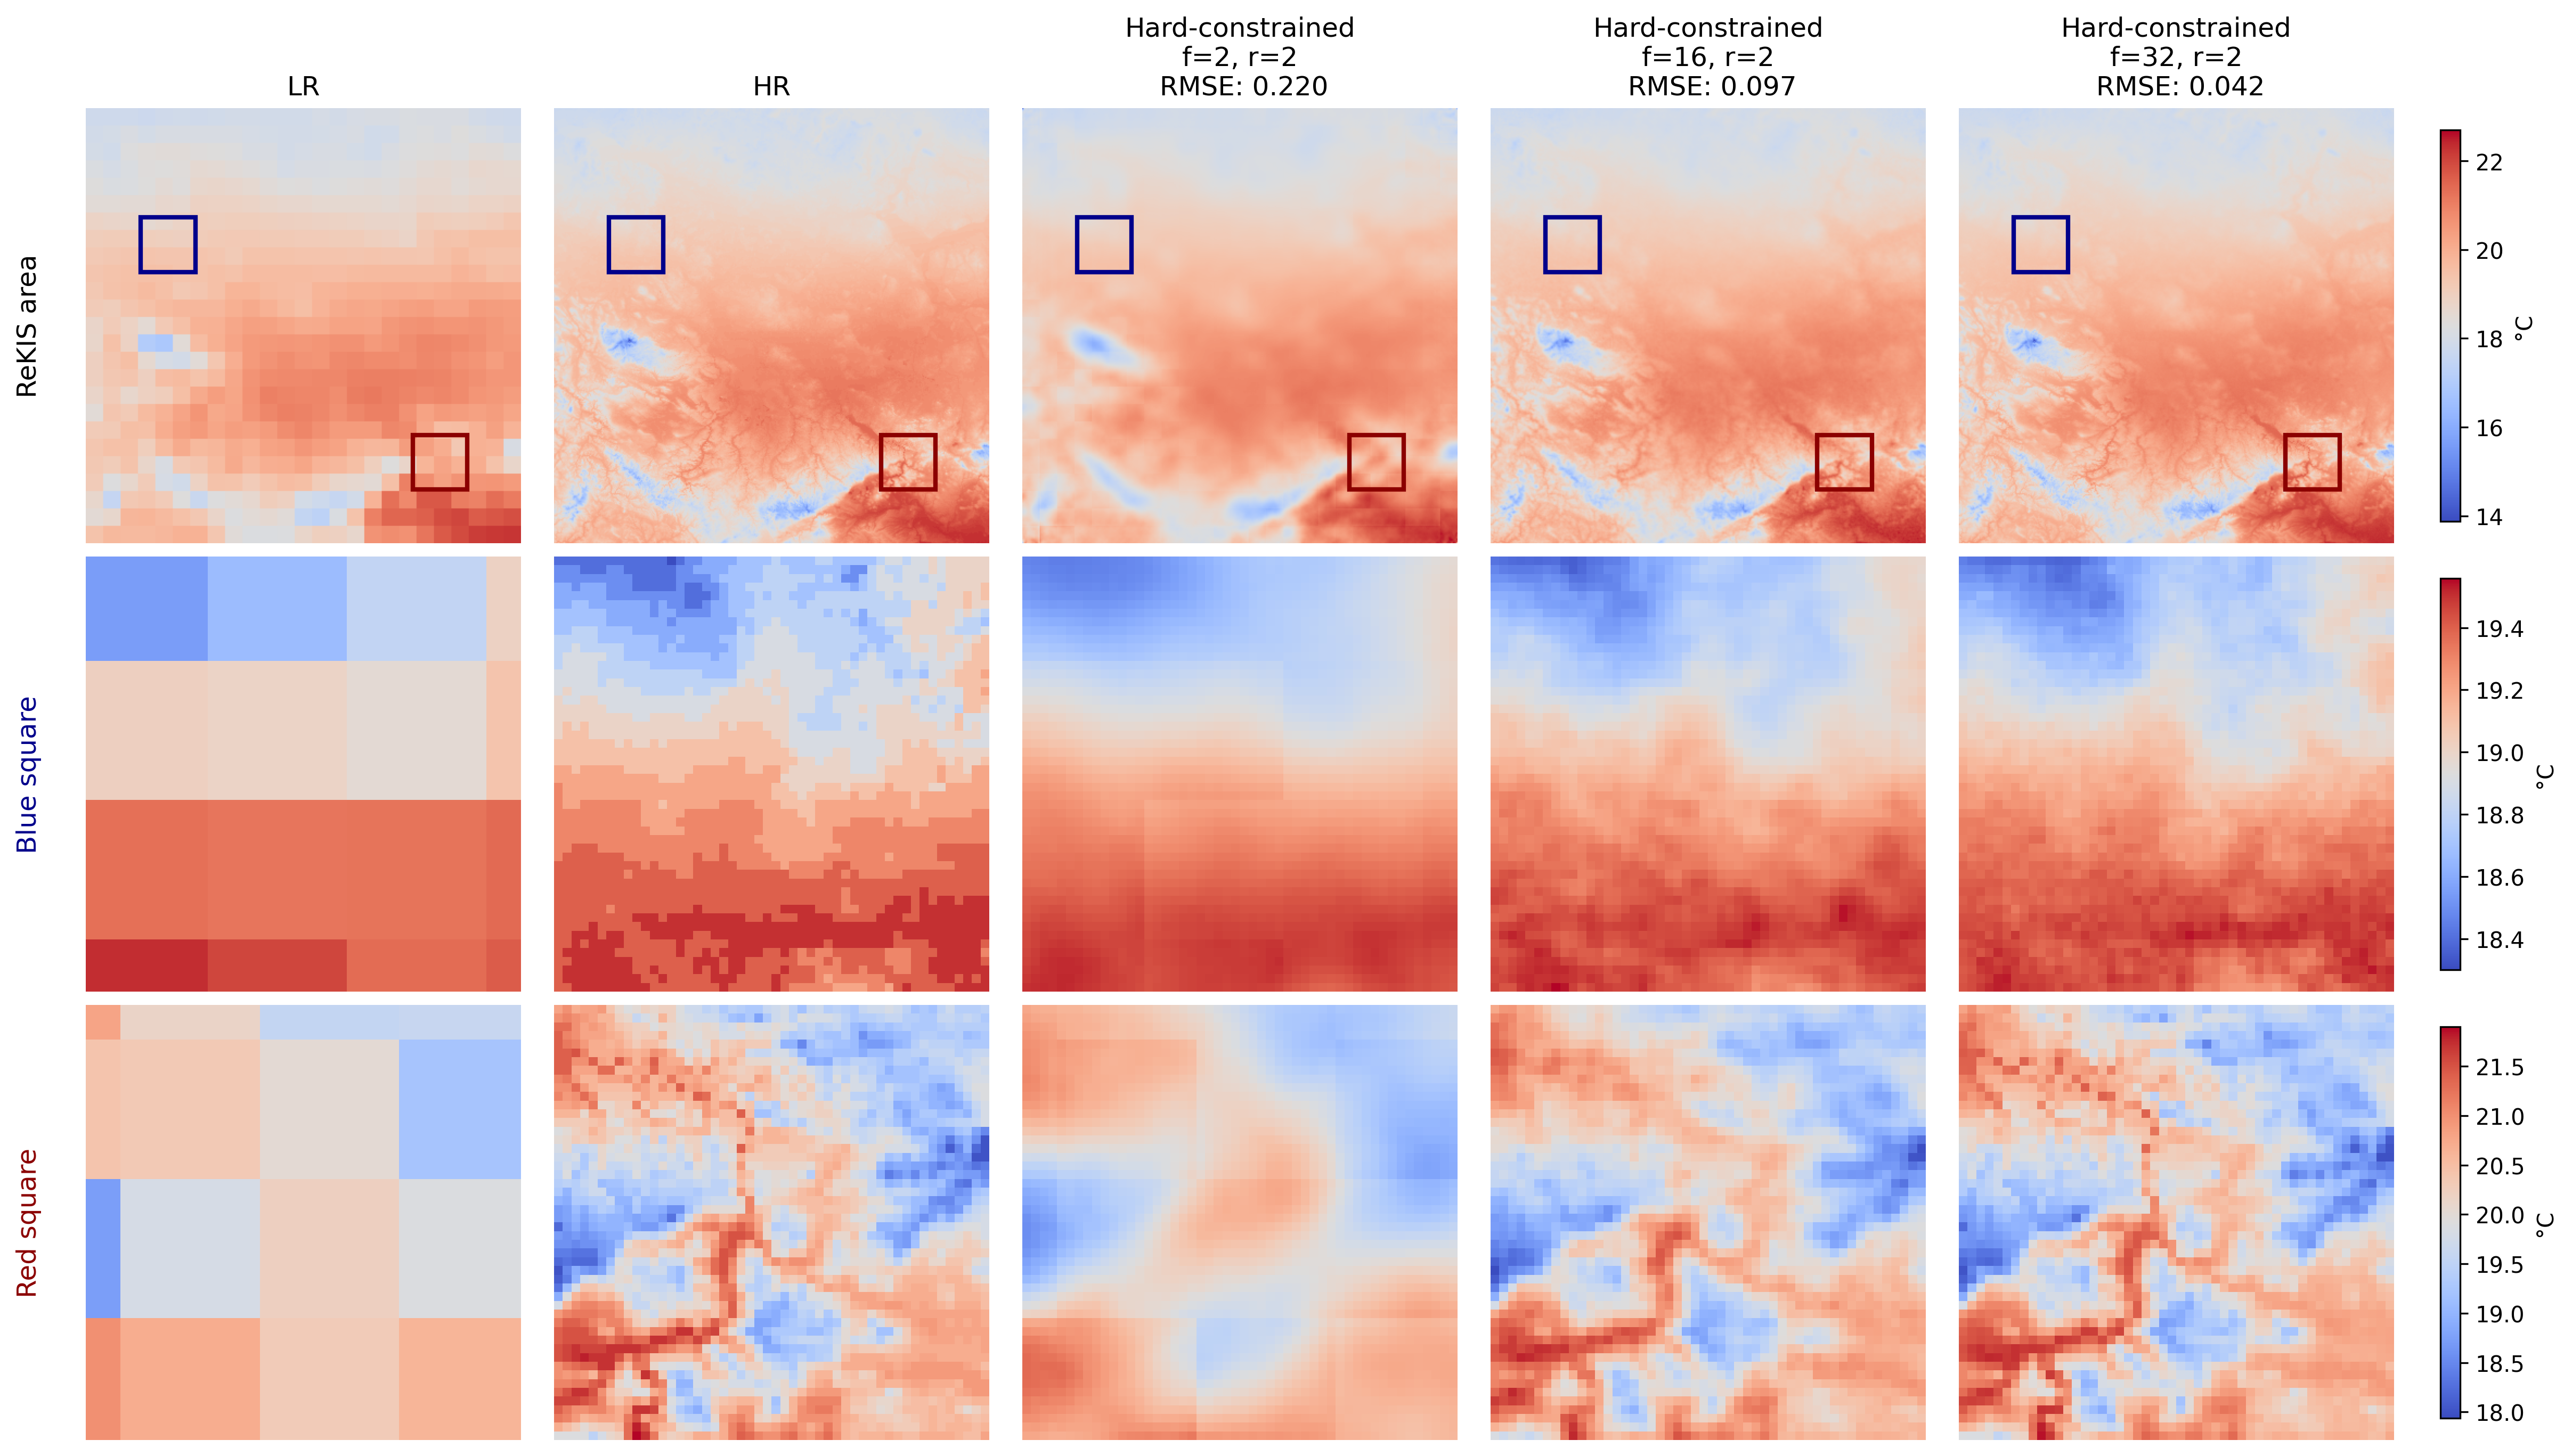
\includegraphics[width=0.88\linewidth]{images/sizes_comp.png}
    \caption[Hard-constrained different sized models -- output visual comparison]{
    Hard-constrained different sized models -- output visual comparison. 
    The models are from Section~\ref{s:models_size_exp}. 
    The smaller model to the left produces blurred images. 
    The more complex the models become, the more sharp their output appears to be.
    Images correspond to the date 2005-08-18.}
    \label{fig:sizes_comp}
\end{figure}
\end{landscape}
